\documentclass[11pt,a4paper]{article}

\usepackage[polish]{babel}
\usepackage[utf8]{inputenc}
\usepackage{polski}
\usepackage[T1]{fontenc}
\usepackage{indentfirst}
\usepackage{wrapfig}    % for wrapping figures, tables

\frenchspacing

%\usepackage{amsmath}
%\usepackage{bm}
\usepackage{gensymb}
%\usepackage{hepnames}
\usepackage{epsfig}
\usepackage{graphics}
\usepackage[shortlabels]{enumitem}
%\usepackage{xspace}
%\xspaceaddexceptions{[]\{\}}

%
%
%fixpagesize
\pagestyle{empty}
\addtolength{\textwidth}{6cm}
\addtolength{\textheight}{5cm}
\addtolength{\evensidemargin}{-3cm}
\addtolength{\oddsidemargin}{-3cm}
\addtolength{\topmargin}{-3cm}
\parindent=0cm


%
%
%small distance in list/item/enum for enumitem package
\setlist[itemize,enumerate]{topsep=0em}
\setlist{noitemsep}

%print zadanie #
\newcounter{zadanie}\newcommand{\zadanie}[1][]{\addtocounter{zadanie}{1} ~\\  {\bf \emph{Zadanie \arabic{zadanie} #1 }} \\}
\newcounter{zaddom}\newcommand{\zaddom}[1][]{\addtocounter{zaddom}{1} ~\\  {\bf \emph{Zadanie domowe \arabic{zaddom} #1 }} \\}
%\renewcommand{\zadanie}[1][]{\pagebreak  ~\\  {\bf \emph{Zadanie }} \\} \addtolength{\topmargin}{-2cm}


%%%%%%%%%%%%%%%%%%%%%%%%%%%%%%%%%%%%%%%%%%%%%%%%%%%%%%
\begin{document}           % End of preamble and beginning of text.

\begin{centering}
\bf{\Large{Termodynamika z elementami fizyki statystycznej}}\\
Ćwiczenia 1 (26 lutego 2024)\\[5mm]
Dochodzenie do równowagi termicznej, rozszerzalność cieplna \\
\end{centering}
\vspace{1mm}

\zadanie
Metalowy blok o temperaturze początkowej $T_1$ umieszczony został
w otoczeniu, którego temperatura przełączana jest regularnie
pomiędzy dwiema ustalonymi wartościami: $T_1$ i $T_2$ ($T_1>T_2$).
Jak zmienia si"e temperatura bloku w funkcji czasu?
Znajdź maksymalną i minimalną temperaturę bloku
w stanie ustalonym (tzn. po bardzo dużej liczbie przełączeń)
i przedyskutuj jako funkcję okresu $b$.
\begin{center}
\resizebox{0.5\linewidth}{!}{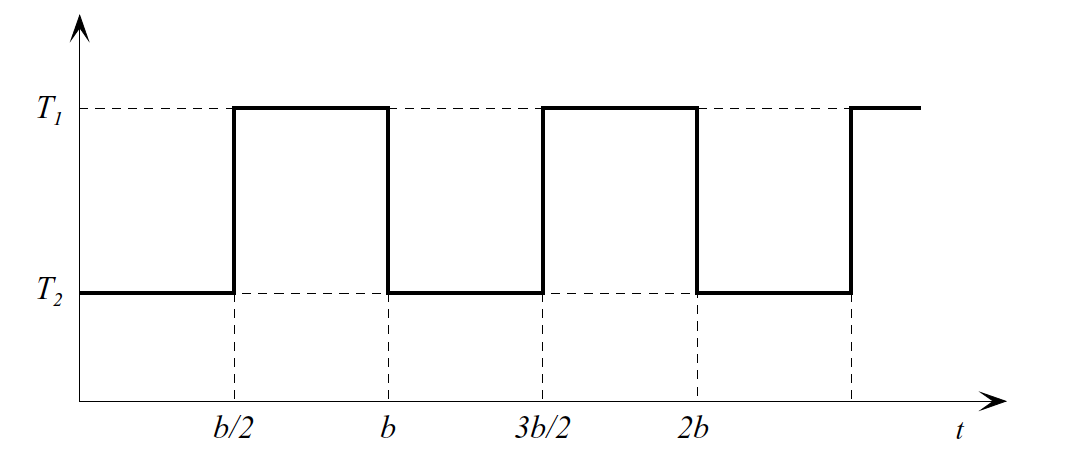
\includegraphics{figure_temp_switching.png}}
\end{center}\vspace{-5mm}
\vskip 10pt
%\textbf{Odpowiedź:} $T_{\rm max} = (T_{1} + T_{2} e^{-\alpha b/2})/(1 + e^{-\alpha b/2})$, $T_{\rm min} = (T_{2} + T_{1} e^{-\alpha b/2})/(1 + e^{-\alpha b/2})$.

\zadanie
Blok metalowy umieszczony jest w otoczeniu, którego temperatura
zmienia się według wzoru:
\[T_{ot}(t) = T_\circ + A \cos(\omega t).\]
Początkowa temperatura bloku wynosi $T_\circ$. Znajdź zależność
temperatury bloku od czasu w stanie ustalonym.
\vskip 10pt
%\textbf{Wskazówka:} Przyjmij, że rozwiązanie r. Newtona jest postaci: $T(t) = C e^{-\alpha t} + K \sin (\omega t) + L \cos (\omega t) + T_0.$
%\textbf{Odpowiedź:} $T(t) = T_{0} + B \sin(\omega t - \phi)$, gdzie $B = \alpha A/\sqrt{\omega^{2} + \alpha^{2}}$ i $\tg \phi = \omega/\alpha$.  

\zadanie
\begin{wrapfigure}{r}{0.3\linewidth}\vspace{-1cm}
\resizebox{\linewidth}{!}{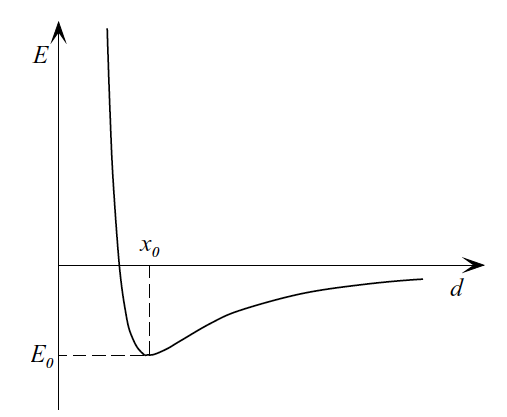
\includegraphics{figure_potencjal.png}}
\end{wrapfigure}
Energia potencjalna oddzia"lywania dw"och atom"ow danej substancji jest
przedstawiona na rysunku obok. Znale"z"c "sredni"a
odleg"lo"s"c mi"edzy atomami odpowiadaj"ac"a energii $E>E_0$,
zak"ladaj"ac, "re:
\begin{enumerate}
\item 
\parbox[t]{\linewidth}{
w pobli"ru punktu r"ownowagi $x=x_0$ energia 
potencjalna daje si"e przybli"ry"c wzorem\\[2mm] 
\centerline{$E_p(x) \approx a (x-x_0)^2 - b (x-x_0)^3 + E_0$,}\\[2mm]
gdzie $a$ i $b$ s"a sta"lymi dodatnimi,
}
\item anharmoniczna poprawka trzeciego rz"edu jest ma"la, tzn. \mbox{$b |x-x_0|\ll a$},
\item punkty zwrotne $x_{\rm min}$ i $x_{\rm max}$
drga"n bardzo niewiele r"o"rni"a si"e od punkt"ow zwrotnych
oscylatora harmonicznego $x^h_{\rm min}$ i $x^h_{\rm max}$ (dla $b=0$),
\item \mbox{średnia odległość międzyatomowa w czasie drgań może być
przybliżona przez średnią} arytmetyczną $\langle x\rangle \approx \frac{x_{\rm min}+x_{\rm max}}{2}$.
\end{enumerate}
\vskip 10pt
%\textbf{Odpowiedź:} $\langle x \rangle \approx x_{0} + b \cdot \Delta E /(2a^{2})$.

\zadanie
Wykaza"c, "re dla materia"lu anizotropowego zachodzi zwi"azek:
$\gamma\,=\,\alpha_1+\alpha_2+\alpha_3$, gdzie $\gamma$ jest wsp"o"lczynnikiem rozszerzalno"sci obj"eto"sciowej danego materia"lu, za"s $\alpha_i ~(i=1,2,3)$
s"a wsp"o"lczynnikami rozszerzalno"sci liniowej wzd"lu"r 3 
nier"ownowa"rnych (i wzajemnie prostopad"lych) kierunk"ow tego materia"lu.

%\textbf{Wskazówka:} Skorzystaj wprost z definicji obu współczynników.

\zadanie
Termometr rt"eciowy sk"lada si"e ze szklanego, kulistego zbiorniczka z rt"eci"a po"l"aczonego ze szklan"a kapilar"a. W temperaturze $T_0=0\degree$C
pole przekroju poprzecznego kapilary wynosi $A_0$,
a zbiorniczek ma obj"eto"s"c $V_0$ i jest ca"lkowicie wype"lniony rt"eci"a. Wsp"o"lczynnik rozszerzalno"sci
obj"eto"sciowej rt"eci wynosi $\beta$, a wsp"o"lczynnik rozszerzalno"sci
liniowej szk"la wynosi $\alpha$. Jaka b"edzie d"lugo"s"c s"lupa rt"eci w kapilarze w temperaturze $T$? Przedyskutuj wynik.
%\textbf{Odpowiedź:} $h = \frac{\Delta V}{A_0} = \frac{V_0}{A_0} (\beta - 3\alpha) \Delta T$.

\zadanie
Odległość między słupami elektrycznymi wynosi 50\,m.
O ile zmienia swoją długość zawieszony między nimi cienki drut miedziany,
jeżeli temperatura zmienia się od -25\degree C do +35\degree C?
Współczynniki rozszerzalności liniowej miedzi wynosi $\alpha = 8.9\cdot 10^{-6} {\rm K}^{-1}$.
Oszacuj zmianę zwisania drutu. Załóż, że na początku drut ma długość równą
odległości między słupami, a w większej temperaturze przyjmuje kształt
jak po obciążeniu na środku ciężarkiem.

\vskip 10pt

%\textbf{Odpowiedź:} $x = \sqrt{\frac{L_0 \Delta L}{2}} \approx 0.82\, {\rm m}$.


%\textbf{Odpowiedź:} $h = \frac{\Delta V}{A_0} = \frac{V_0}{A_0} (\beta - 3\alpha) \Delta T$.


\vspace*{5mm}
\begin{centering}
\bf{ Zadania domowe } \\[1mm]
\end{centering}

\zaddom 
Blok metalowy znajduje się w otoczeniu
którego temperatura zmienia się w czasie zgodnie z wzorem:\\
\[T_1=T_0+A\exp(-\beta t),\] gdzie stałe $A,\beta>0$. 
Temperatura początkowa bloku wynosi $T_0$. Znależć zależność
temperatury bloku od czasu i przedyskutować ją jako funkcję
$\beta$. Po jakim czasie blok osiągnie maksymalną
temperaturę?

\vskip 10pt

\textbf{Odpowiedź:} Temperatura bloku w chwili $t$ wynosi $T(t) = T_0 + \frac{Ak}{k - \beta}\left(e^{-\beta t} - e^{-kt}\right)$.


\zaddom
Blok metalowy o temperaturze początkowej $T_0$ umieszczono na czas $t_1$ w otoczeniu,
którego temperatura wynosi $T_0-\Delta T$. Na jaki czas $t_2$ należy umieścić następnie blok
w otoczeniu o temperaturze $T_0+\Delta T$, aby znów osiągnął temperaturę $T_0$?
Czy wynik zależy od $\Delta T$? 
Zbadaj wynik w granicach $t_1\rightarrow 0$ i $t_1\rightarrow \infty$. 
Który z czasów jest krótszy: $t_1$ czy $t_2$?

\vskip 10pt

\textbf{Odpowiedź:} $t_2 = \frac{1}{k} \ln \left(2 - e^{-k t_1}\right)$. 

\zaddom
W lodówce, w temperaturze $0^\circ$C przechowywana jest butelka coli.
Zmierzono, że w godzinę po wyjęciu jej z lodówki i pozostawieniu w otoczeniu o
temperaturze $20^\circ$C temperatura płynu osiąga $14^\circ$C.
\begin{enumerate}[a)]
\item Ile wynosi czas relaksacji temperatury w tej sytuacji?
\item Na ile minut przed otwarciem butelki należy wyjąć colę z lodówki, jeżeli
chcemy aby miała ona optymalną do picia temperaturę $4^\circ$C?
\end{enumerate}

\vskip 10pt

\textbf{Odpowiedź:} a) czas relaksacji $\tau \approx 50\, {\rm min}$, b) czas ogrzewania do optymalnej temperatury $t \approx 11\, {\rm min}$. 


\zaddom 
Punktowa masa $m$ drga w jednym wymiarze w polu sił zachowawczych
z energią potencjalną  \linebreak \mbox{$E_p(x) = D \left(e^{-a(x-x_\circ)}-1\right)^2$.}
Jest to tzw. potencjał Morse’a, oddający podstawowe własności potencjałów cząsteczkowych.
Zbadaj jak punkty zwrotne takiego oscylatora zależą od energii całkowitej, która nieznacznie
przekracza minimalną energię potencjalną. W tym celu rozwiń funkcję $E_p(x)$
w szereg Taylora wokół minimum, a następnie zachowaj tylko pierwszy nieznikający człon anharmoniczy. 
Ponadto załóż, że punkty zwrotne niewiele różnią się od rozwiązania dla oscylatora harmonicznego.

\vskip 10pt

\textbf{Odpowiedź:} Punkty zwrotne wynoszą $x_{\pm} = x_0 \mp \frac{\sqrt{E_c/D}}{a} + \frac{E_c/D}{2a}$. 

\zaddom
Jakie długości w temperaturze $T_1 = 0^\circ$C powinny mieć dwa pręty: stalowy i miedziany,
aby w dowolnej temperaturze pręt stalowy był dłuższy od pręta miedzianego o $d = 5\,$cm?
Współczynnik rozszerzalności liniowej dla stali wynosi
$\alpha_{\rm{stali}} = 1.2\cdot10^{-5}\,{\rm K}^{-1}$, a dla miedzi
$\alpha_{\rm{miedzi}} = 1.6\cdot 10^{-5}\,{\rm K}^{-1}$.
Założyć, że współczynniki te nie zależą od temperatury.

\vskip 10pt

\textbf{Odpowiedź:} $L_{0, {\rm stal}} = 20\,{\rm cm}$, $L_{0, {\rm miedź}} = 15\,{\rm cm}$.

%\pagebreak
%\renewcommand{\zaddom}[1][]{ {\bf \vspace*{5mm} \emph{Zadanie }\\} }
%
%
%\zaddom Blok metalowy o temperaturze początkowej $T_0$ umieszczono na
%czas $t_1$ w otoczeniu, którego temperatura wynosi
%$T_0 - \Delta T$. Na jaki czas $t_2$ należy umieścić
%następnie blok w otoczeniu o temperaturze $T_0 + \Delta T$ aby znów
%osiągnął temperaturę $T_0$ ? Pokaż, że wynik
%nie zależy od $\Delta T$. Zbadaj wynik w granicach
%$t_1 \rightarrow 0$, $t_1 \rightarrow \infty$. Który z
%czasów jest krótszy : $t_1$ czy $t_2$ ?
%
%\zaddom Kulę metalową o temperaturze początkowej $T_0$ umieszczono
%w otoczeniu o tempe\-raturze $T_0 - \Delta T$ ($\Delta T > 0$).
%Po czasie $t_1$ umieszczono ją w otoczeniu o
%temperaturze $T_0 - 2\, \Delta T$. Po jakim czasie temperatura
%kuli osiągnie wartość $T_0 - \Delta T$ ?
%
%\zaddom Kulę metalową umieszczono w otoczeniu, którego temperatura rośnie
%jedno\-stajnie z czasem zgodnie z zależnością : $T_1(t) = T_0 + \alpha t$.
%Początkowa temperatura kuli wynosi $T_0 + T_2$ ($T_2 > 0$). Znajdż zależność
%temperatury kuli od czasu. Kiedy kula osiągnie minimalną temperaturę ?
%
%\zaddom Mam butelkę piwa o temperaturze $20^\circ$C. Wiem z
%wcześniejszych pomiarów, że jeżeli wstawię je do
%lodówki, w której panuje temperatura $0^\circ$C, to po 90
%minutach osiągnie ono moją ulubioną temperaturę
%$5^\circ$C. Dzisiaj jednak bardzo się spieszę, postanowiłem
%więc wstawić piwo do zamrażarki, w kórej panuje
%temperatura $-10^\circ$C. Po jakim czasie powinienem je wyjąć ?
%Ile wynosi czas relaksacji temperatury butelki ?
%
%\zaddom W lodówce, w temperaturze $0^\circ$C przechowywana jest butelka
%wina. Zmierzono, że w godzinę po wyjęciu jej z lodówki
%i pozostawieniu w otoczeniu o temperaturze $20^\circ$C temperatura
%wina osiąga $14^\circ$C. Ile wynosi czas relaksacji temperatury w tej sytuacji?
%Na ile minut przed otwarciem butelki należy wyjąć ją z
%lodówki, jeżeli chcemy aby wino miało optymalną do picia
%temperaturę $4^\circ$C?
%
%\zaddom W lodówce, wewnątrz której panuje temperatura $T_1$,
%znajduje się kostka masła o tej samej temperaturze.
%Lodówka stoi w otoczeniu o stałej temperaturze $T_0 > T_1$.
%W chwili $t = 0$ wyłączono prąd i lodówka przestała
%działać. Znajdż zależność temperatury masła
%od czasu. Załóż, że wyrównywanie temperatur zarówno w
%układzie wnętrze lodówki--jej otoczenie, jak i w układzie
%masło--jego otoczenie zachodzi zgodnie z newtonowskim prawem
%ostygania ze znanymi czasami relaksacji $\tau_1$ i $\tau_2$.
%Kostka masła jest znacznie mniejsza od lodówki.
%
%\zaddom W letni dzień, przy temperaturze powietrza $T_0 = 30^\circ$C
%kupiłem w sklepie butelkę wody mineralnej. Zakupiona woda, wyjęta
%ze sklepowej lodówki, miała temperaturę $T_1 = 4^\circ$C.
%Po dojściu do domu, co zajęło mi 20 minut, natychmiast
%wstawiłem wodę do domowej lodówki, w której panuje
%temperatura $T_2 = 0^\circ$C i zostawiłem w niej na kolejne 20
%minut. Oblicz końcową temperaturę wody jeżeli wiadomo,
%że czas relaksacji temperatury w układzie butelka-otoczenie
%wynosi 40 minut.
%
%

\end{document}
